\documentclass{article}
\usepackage[spanish]{babel}   
\usepackage[numbers,sort&compress]{natbib}
\usepackage{float}
\usepackage{listings}
\usepackage{graphicx} 	% Nos permite importar imagenes 
\usepackage{subfigure}
\usepackage[left=3cm,right=3cm,top=3cm,bottom=3cm]{geometry}

%-------------------------- Por si se romple la URL --------------------------
\usepackage[hyphens]{url}
\usepackage[hidelinks]{hyperref}
\hypersetup{breaklinks=true}	
\urlstyle{same}
\usepackage{cite}
%-------------------------- Por si se romple la URL --------------------------

\title{Reporte Tarea 10}
\author{Victor Alejandro Oviedo Martínez}



\begin{document}
\maketitle
\hrule

\section{Introduccón}\label{intro}
Para esta décima tarea \citep{DRA.P10} se ha estudiado el tema algoritmo genético, el cual podemos decir, es una técnica para encontrar la  solución a problemas complejos de los cuales no contamos con un modelo preciso para encontrar la solución optima. Esto será aplicado al problema de la mochila, el cual es un problema de optimización en donde tendremos una cantidad de objetos con dos características; valor y peso. En donde la mochila tiene una capacidad de peso, el objetivo es encontrar la mejor combinación  de objetos con el mayor valor posible, y ademas, que el peso total de estos objetos no superen la capacidad de la mochila.\\ 




\section{Desarrollo}

Para esta novena tarea se ha planteado el siguiente problema: Cambia la selección de padres para reproducción a que use selección de ruleta: cada solución se selecciona como padre con una probabilidad que es linealmente proporcional a su valor de función objetivo y a su factibilidad, combinando los dos a alguna función que parezca conveniente.\\

Genere instancias con tres distintas reglas:


\begin{enumerate}
\item El peso y el valor de cada objeto se generan independientemente con una distribución exponencial,
\item El peso de cada objeto se generan independientemente con una distribución exponencial y su valor es (positivamente) correlacionado con el peso, con un ruido normalmente distribuido de baja magnitud,
\item El peso de cada objeto se generan independientemente con una distribución exponencial y su valor es inversamente correlacionado con el peso, con un ruido normalmente distribuido de baja magnitud.
\end{enumerate}


Determina para cada uno de los tres casos a partir de qué tamaño de instancia el algoritmo genético es mejor que el algoritmo exacto en términos de valor total obtenido por segundo de ejecución y si la inclusión de la selección de ruleta produce una mejora estadísticamente significativa.\\

Para el desarrollo de esta tarea se a utilizado el código ejemplo proporcionado por \citet{DRA.Code}, el cual implementa la técnica de algoritmo genético para apreciar en un tiempo determinado de simulación el mejor valor generado por el algoritmo, esto con el fin de comparar el valor optimo previamente calculado contra el mejor valor generado del algoritmo.\\  

Para la edición de este código se ha iniciado generado las funciones necesarias para tener las tres instancias diferentes; \texttt{generador-pesos}, \texttt{generador-valores}, \texttt{generador-pesos2}, \texttt{generador-valores2},
\texttt{generador-pesos3}, \texttt{generador-valores3},
\texttt{generador-pesos4}, \texttt{generador-valores4}. Dado que se tienen diferentes instancias se ha creado del mismo modo funciones para la simulación de estas instancias; \texttt{simu()}, \texttt{simu2()}, \texttt{simu3()}, \texttt{simu4()}. En estas funciones lo que se tiene es el código donde se simula con una cantidad de objetos (\texttt{n}), en donde una vez dado la cantidad de objetos (\texttt{n}) calcula el tiempo que se tarda en generar la respuesta optima. Después se realizan las iteraciones y en cada iteración se toma el tiempo que tardó en generar la respuesta, esto es comparado contra el tiempo de la respuesta optima, lo que se busca es ver si se tiene un mejor respuesta en términos de valor total obtenido por segundo de ejecución,  de no comprobar esta respuesta y  sobrepasar el tiempo de la respuesta optima la simulación terminaría. Por lo tanto, se repetiría la simulación pero ahora con un cantidad de objetos (\texttt{n}) mayor, esto hasta encontrar el mejor tiempo de respuesta en términos de valor total obtenido por segundo de ejecución. A la vez este procedimiento se repite cuarenta veces para tener una muestra de la simulación en curso. 

\begin{lstlisting}[language=Python]
for k in range(2):
    for l in range(4):
        for i in range(40):
            for n in range(10,100):
            
                if l == 0:
                    exp = []
                    exp = simu(n,k)
                    if exp != None:
                        if exp[0] == 123:
                            if k == 0:
                                expts.append(exp[1])
                                break
                            if k == 1:
                                exptsk.append(exp[1])
                                break
\end{lstlisting} 

En la tarea se tiene la especificación de repetir tres instancias diferentes, sin embargo se ha decidido dejar la instancia del ejemplo de \citet{DRA.Code}, por lo tanto sé tendrán cuatro instancias diferentes. Por último, dado que uno de los objetivos es comparar el método con ruleta y  sin ruleta con las mismas instancias, se agrega un \texttt{for} el cual nos ayuda a utilizar el mismo código para simular con y sin ruleta. Por último, se grafican los resultados de todas las simulaciones.



\section{Conclusión}

Cómo metodo ilustrativo a lo que se simula en esta tarea, se tiene la figura \ref{f1} en la cual podemos ver cuatro diferentes ejemplos en donde la linea verde marca el valor optimo generado, en azul se traza el comportamiento que tuvo la simulación sin ruleta, y en rojo el comportamiento de la simulación con ruleta. Es importante ver el comportamiento de estas imágenes y compararlas entre si, ya que viendo esto podemos ver el rango comportamiento que posible mente tendremos en la simulación con las diferentes instancias.\\

En cuanto a la figura \ref{f2} tenemos los resultados con las tres instancias pedidas mas la instancia del ejemplo de \citet{DRA.Code}, en donde para cada instancia se simuló 40 veces y a esto tendremos como resultado 40 datos con la mejor respuesta en términos de valor total, obtenido por segundo de ejecución. 

\begin{figure}[H]
\centering
\subfigure[Ejemplo 1.]{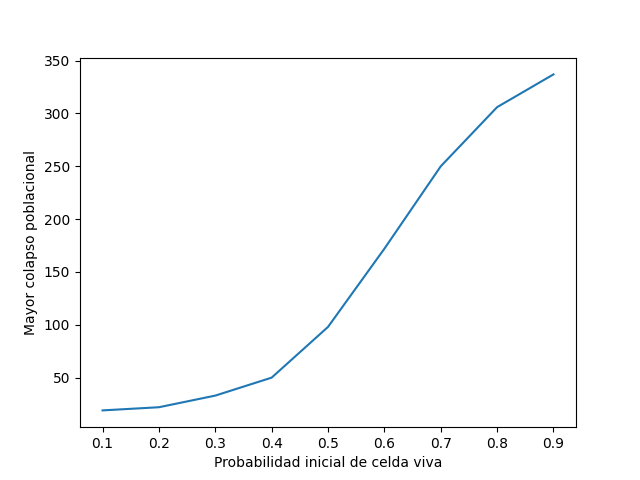
\includegraphics[width=75mm]{/Users/victor/Desktop/Figure_1.png}}
\subfigure[Ejemplo 2.]{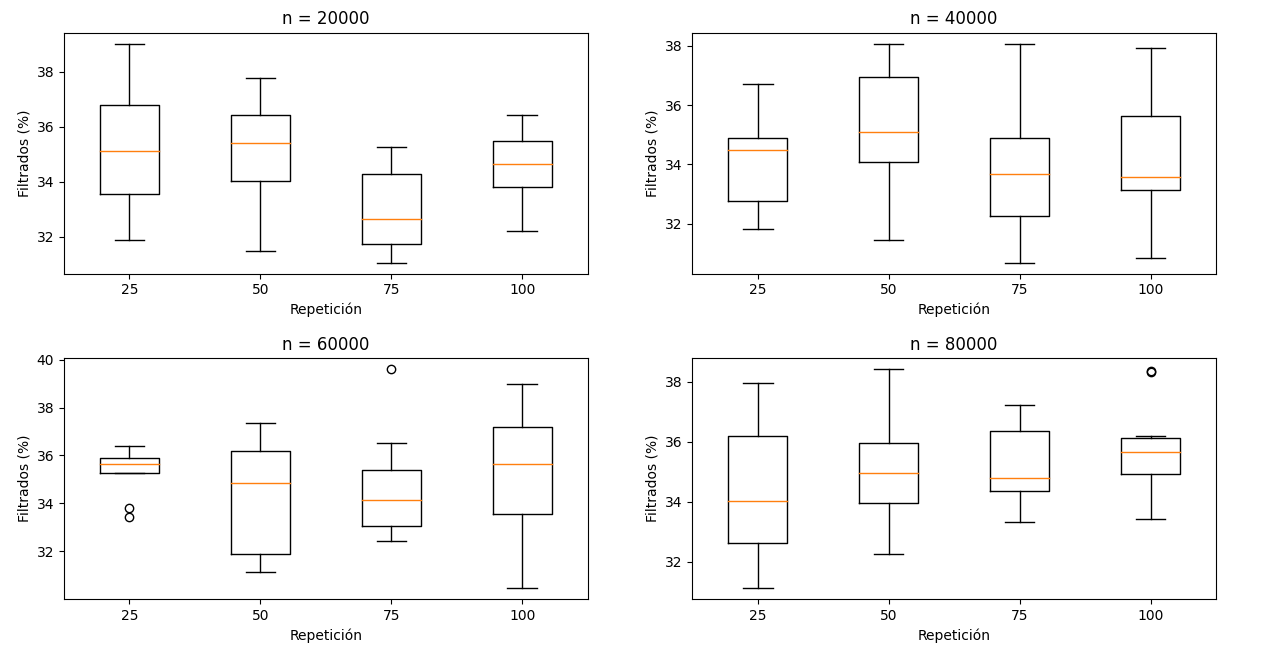
\includegraphics[width=75mm]{/Users/victor/Desktop/Figure_2.png}}
\subfigure[Ejemplo 3.]{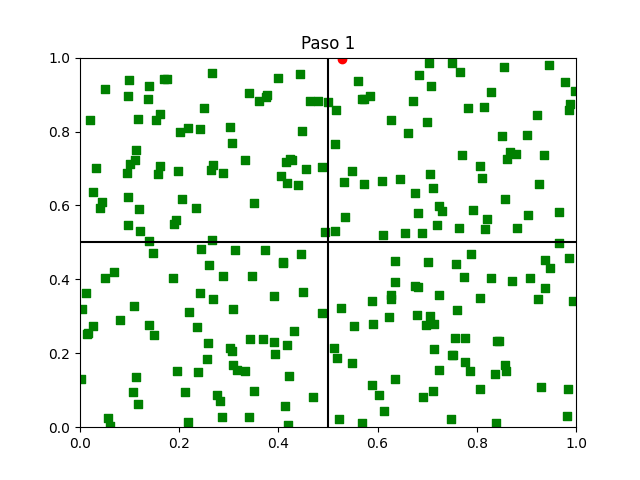
\includegraphics[width=75mm]{/Users/victor/Desktop/Figure_3.png}}
\subfigure[Ejemplo 4.]{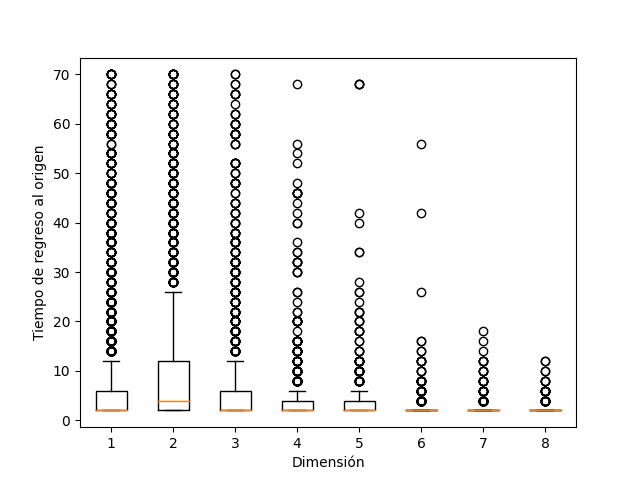
\includegraphics[width=75mm]{/Users/victor/Desktop/Figure_4.png}}
\caption{Ejemplos ilustrativos.} 
\label{f1}
\end{figure}

\begin{figure}[H]
\begin{center}
	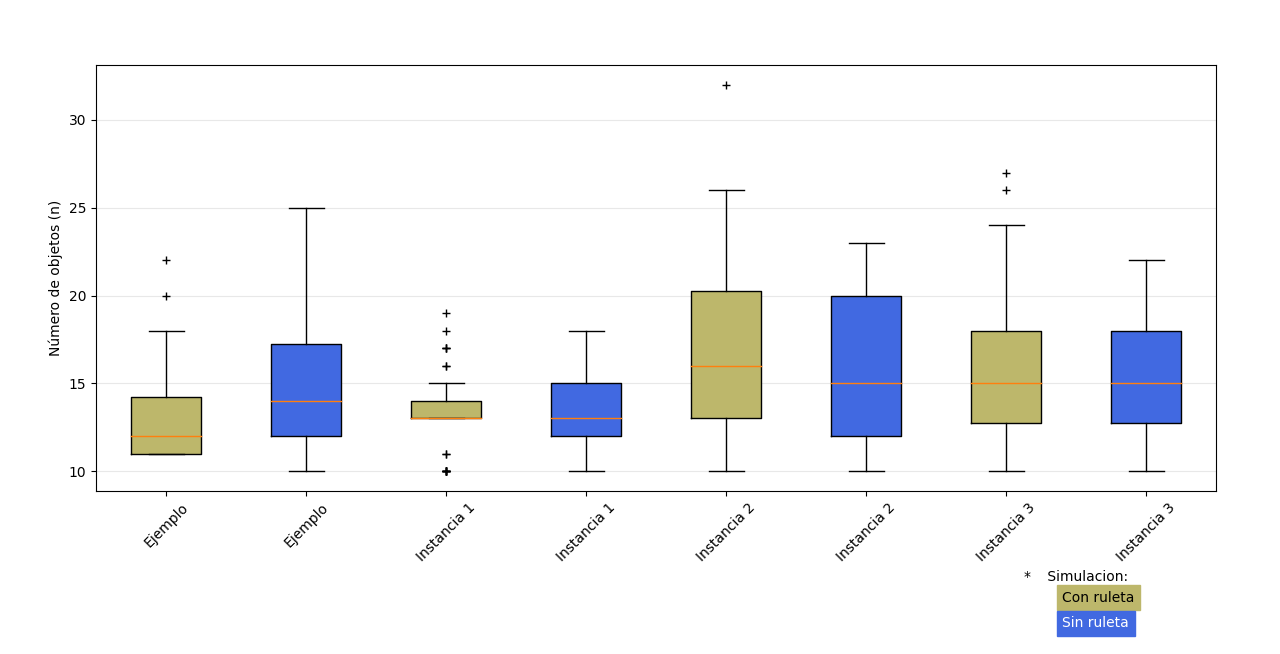
\includegraphics[height=3.05in]{/Users/victor/Desktop/Figure_5.png}
	\caption{ Simulación con las diferentes instacias, 40 repeticiones.}
	\label{f2}
\end{center}
\end{figure}

Cómo conclusión a esta tarea, y con base en los datos obtenidos no se puede afirmar que el método de la ruleta aporte una mejora significativa, ya que por ejemplo, en los ejemplos de la figura \ref{f1} no siempre se observa un mejor comportamiento del método de ruleta, mas bien este refleja comportamientos similares al método sin ruleta, y en ocaciones este es mejor y también peor. En cuando a los resultados de la figura \ref{f2}, tenemos que para las simulación de Ejemplo y Instancia 1 el método de la ruleta es mejor, sin embargo para para las simulación de Instancia 2 y Instancia 3 el método con ruleta parecería ser peor, tomando en cuenta que la media de las simulaciones de Instancia 3 son la misma y la diferencia no es tan grande.
%-------------------------- Por si se rompe la URL --------------------------
\Urlmuskip=0mu plus 1mu\relax
%-------------------------- Por si se rompe la URL --------------------------
\bibliography{ref.Tarea10.bib}
\bibliographystyle{plainnat}

\end{document}